\documentclass{article}

\usepackage{booktabs}
\usepackage{tabularx}
\usepackage{hyperref}
\usepackage{multirow}
\usepackage{graphicx}
\usepackage{float}
\usepackage{geometry}
\usepackage{soul}
\usepackage{ulem}
\geometry{margin = 0.75in}

\hypersetup{
    colorlinks=true,       % false: boxed links; true: colored links
    linkcolor=red,          % color of internal links (change box color with linkbordercolor)
    citecolor=green,        % color of links to bibliography
    filecolor=magenta,      % color of file links
    urlcolor=cyan           % color of external links
}
\title{Hazard Analysis\\Digital Twin Forest}

\author{Team 8, Forest Mirror
		\\ Yichen Jiang, jiany34
		\\ Bowen Zhang, zhangb82
		\\ Junhong Chen, chenj297
		\\ Jiacheng Wu, wuj187
		\\ Tingyu Shi, shit19
}

\date{}


\begin{document}


\maketitle
\thispagestyle{empty}

\pagenumbering{roman}

\begin{table}[hp]
\caption{Revision History} \label{TblRevisionHistory}
\begin{tabularx}{\textwidth}{llX}
\toprule
\textbf{Date} & \textbf{Developer(s)} & \textbf{Change}\\
\midrule
October 18 & All team members & Initial documents\\
\bottomrule
\end{tabularx}
\end{table}




~\newpage

\tableofcontents
\listoftables
\listoffigures
\cleardoublepage

\pagenumbering{arabic}

\section{Introduction}

This document is the hazard analysis of the project Digital Twin Forest. Digital twin forest is a virtual representation of the natural world, specifically a real forest. The detailed introduction of our project can be found \href{https://github.com/wuj187/DigitalTwinCAS/blob/main/docs/ProblemStatementAndGoals/ProblemStatement.pdf}{here}.

\section{Scope and Purpose of Hazard Analysis}

The scope of this document is to analyze and identify the hazards may occur
in our system 
in order to minimize the cost and harm of them when they occur.\\

\noindent Safety is always the top requirement of ours. Though we are developing a software which may not lead to any physical harms to our users, we would make an effort to examine and then avoid any other kind of possible harms. We care about not only our users but also our development and maintenance team, which will
provide long-term support for our users.\\

\noindent The purpose of our product is to display visualized 
forest information to users. As a result, users would be able to better make their
strategies based on the information we provided in the product, which means,
inaccurate data might mislead the users when making decisions. Thus, different
with many other products, the information accuracy is another one of our top
concerns. Regarding to the purpose of the product and the requirements of
information accuracy, we will also include the analysis of possible source of data
inaccuracy in this document. \\

\noindent With the hazard analysis recorded in this document, we expect our
product to avoid mentioned possible hazards and provide a safer using experience
for our users. 100\% safety is not achievable in a project. However, we believe
that it is still essential to avoid predictable unsafe situations and try our best
to prepare for unpredictable ones. In this document of hazard analysis, it
identifies unsafe behaviours while accomplishing the application, and it makes
sure such behaviours are eliminated. We would raise several recommended actions
for each hazard we mentioned, which provides possible solutions to avoid hazards. 

\newpage

\section{System Boundaries and Components}
\subsection{System Boundaries}
Our system includes the following contents:
\begin{itemize}
    \item Entire application
    \item Computers or laptops that execute our application
    \item Mobile devices like iPad that execute our application
    \item backup data files
\end{itemize}
\subsection{System Components}
The application will be divided into the following 5 components, in order of importance:
\begin{enumerate}
    \item Data collection and analysis
    \item Model construction
    \item Data presentation
    \item Data storage
    \item Future update and maintenance 
\end{enumerate}
\noindent The following is the justification of our components division:\\
As the functions and the whole system of our product are integrated,
dividing components according to the different features or subsystems seems
unreasonable in this case. In contrast, we divide the components regarding to
the development phases, which cover data collection and analysis, model construction, code implementation(including data
presentation and storage), future update and maintenance. In each phase, there are several possible hazards which
might lead to safety and security concerns or data inaccuracy. 

\section{Critical Assumptions}

We assume the data stored in data store classes should always match the data
collected.

\newpage

\section{Failure Mode and Effect Analysis}

\begin{figure}[H]
\begin{flushleft}
\begin{center}
    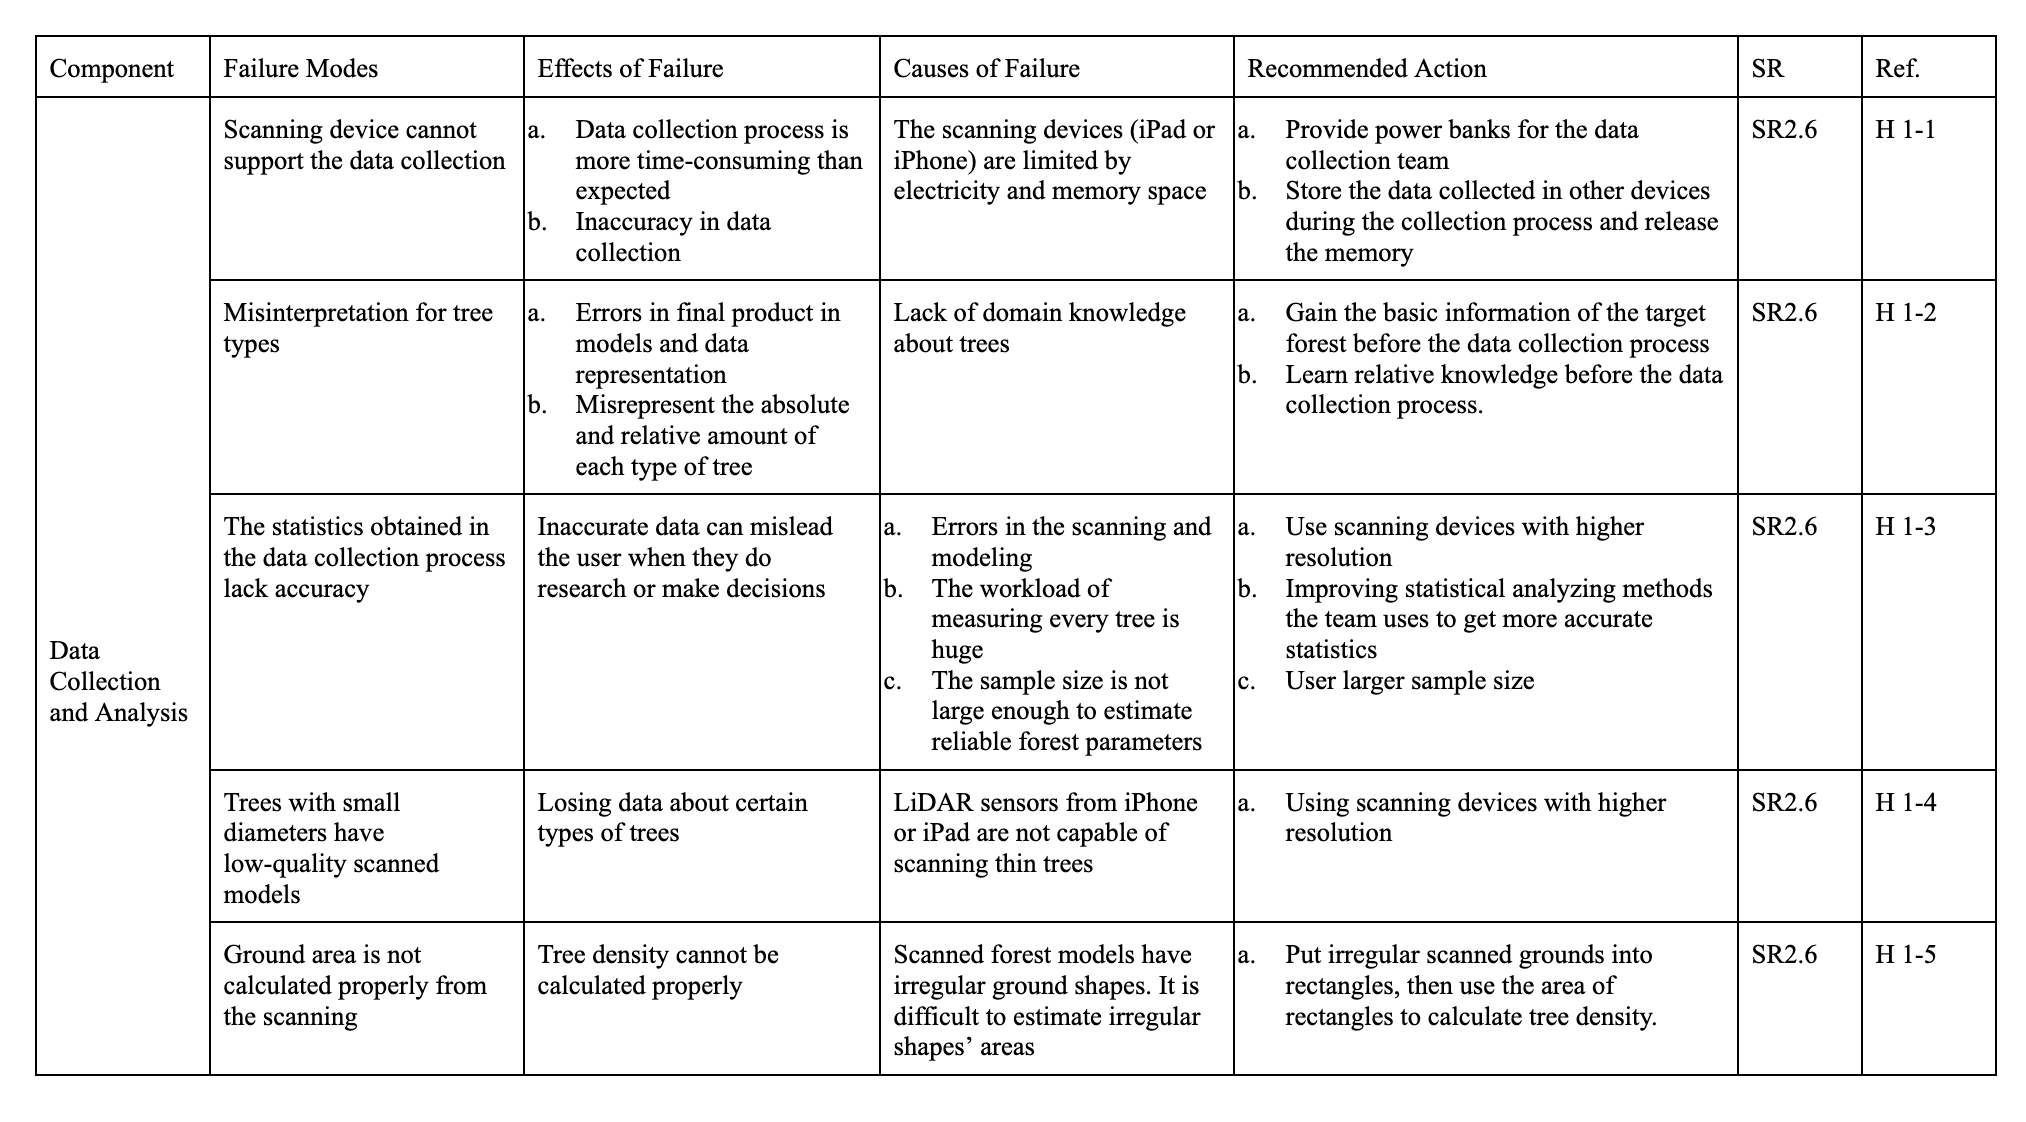
\includegraphics[scale = 0.55]{HA_Pictures/Data_CA.png}
\end{center}
    \caption{FMEA for Data Collection and Analysis}
    \end{flushleft}
\end{figure}

\begin{figure}[H]
\begin{flushleft}
\begin{center}
    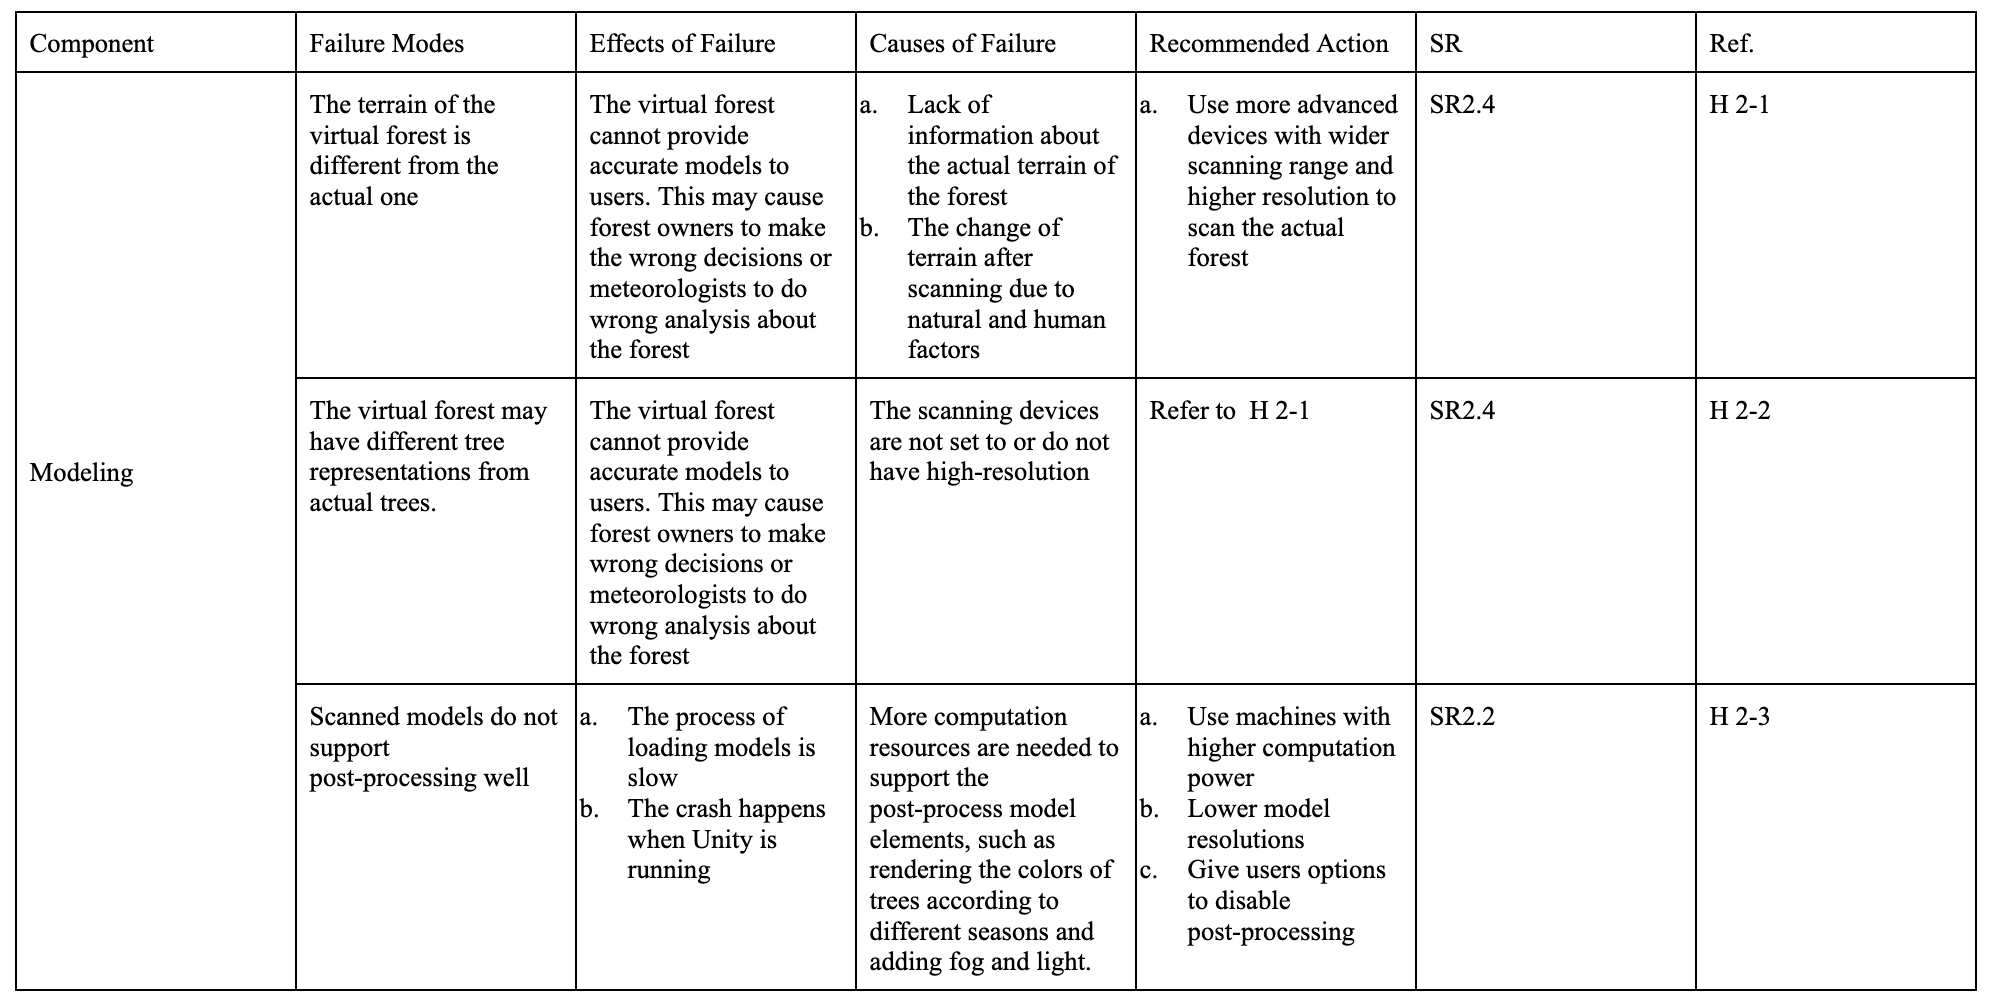
\includegraphics[scale = 0.55]{HA_Pictures/Modeling.png}
\end{center}
    \caption{FMEA for Modeling}
    \end{flushleft}
\end{figure}

\begin{figure}[H]
\begin{flushleft}
\begin{center}
    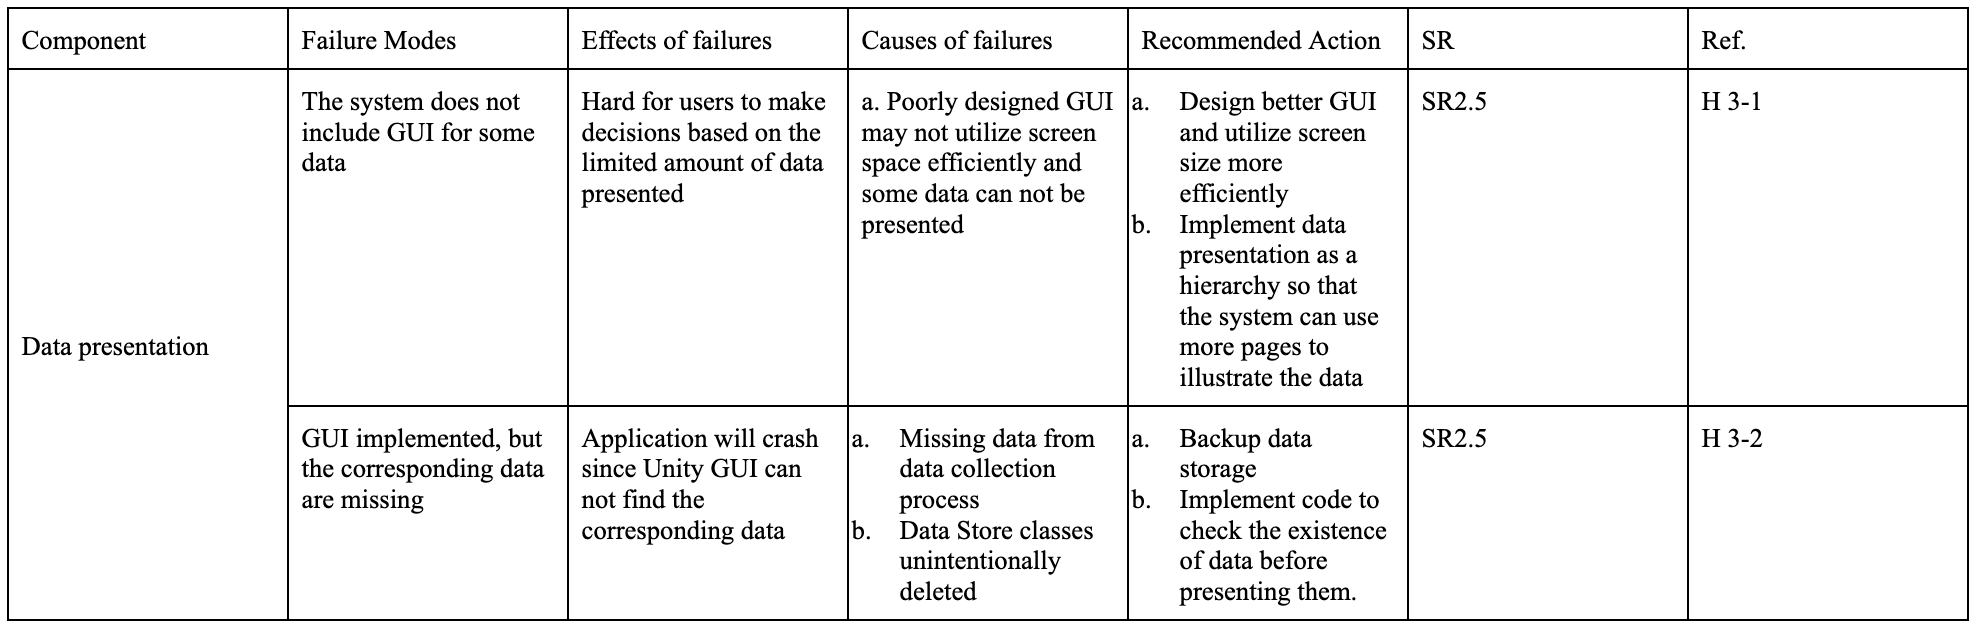
\includegraphics[scale = 0.55]{HA_Pictures/Data_P.png}
\end{center}
    \caption{FMEA for Data Presentation}
    \end{flushleft}
\end{figure}


\begin{figure}[H]
\begin{flushleft}
\begin{center}
    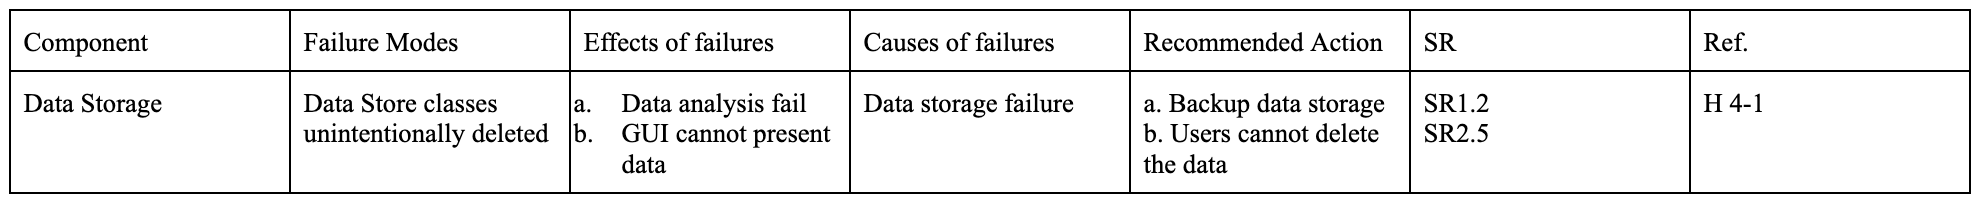
\includegraphics[scale = 0.55]{HA_Pictures/Data_S.png}
\end{center}
    \caption{FMEA for Data Storage}
    \end{flushleft}
\end{figure}

\begin{figure}[H]
\begin{flushleft}
\begin{center}
    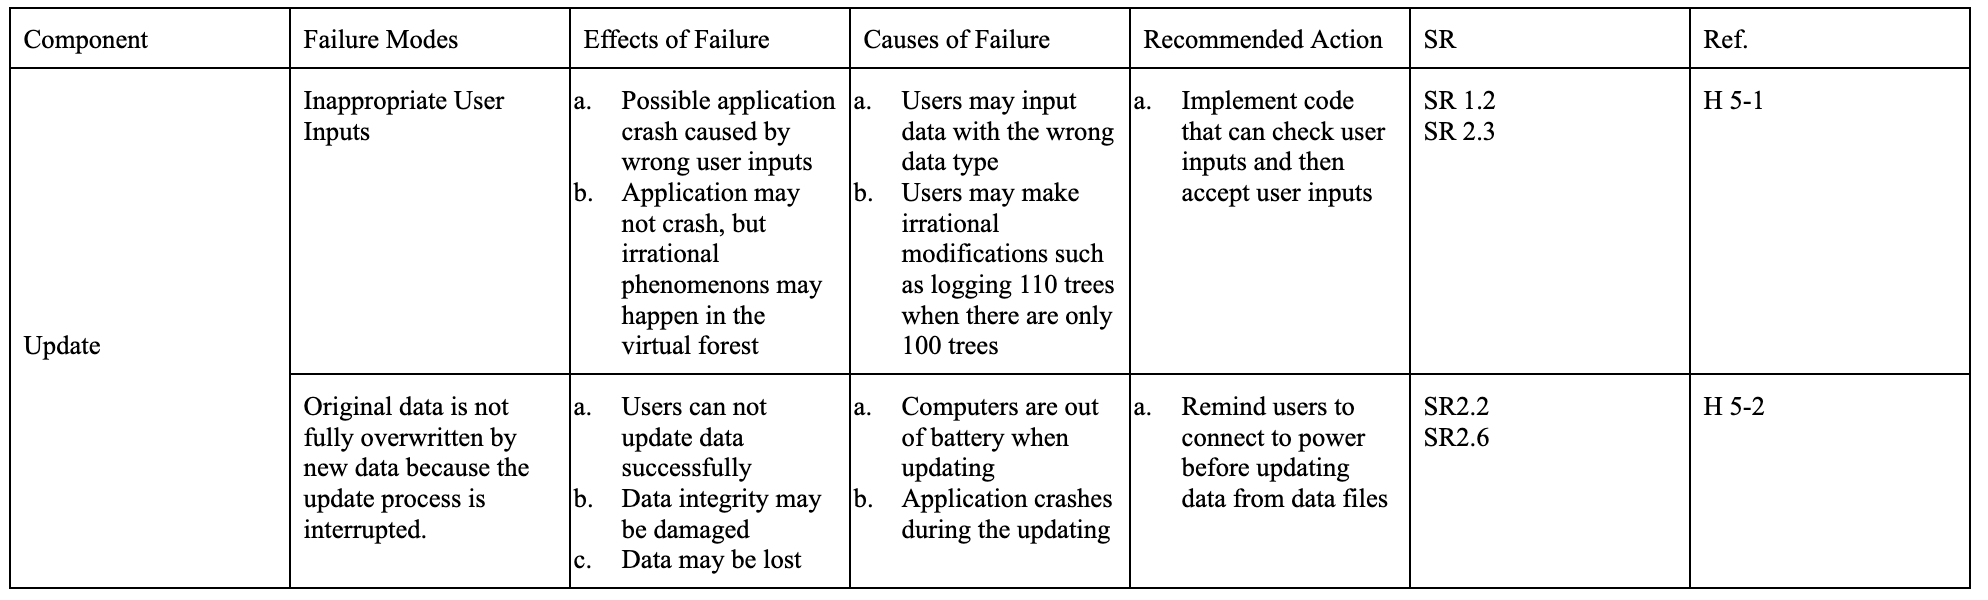
\includegraphics[scale = 0.55]{HA_Pictures/Update.png}
\end{center}
    \caption{FMEA for Data Update}
    \end{flushleft}
\end{figure}

\newpage

\section{Safety and Security Requirements}

New added requirements are shown in \textcolor{blue}{blue} and will be
updated into SRS document. 

\subsection{Access Requirements}
\begin{enumerate}
    \item[SR1.1] The product shall only be accessed by users who download the product from our website.
    \item[\textcolor{blue}{SR1.2}] \textcolor{blue}{Tree and forest
    data shall only be modified through the interface provided by developers.}
\end{enumerate}

\subsection{Integrity Requirements}
\begin{enumerate}
    \item[SR2.1] The system shall not propagate errors throughout the users' devices in case of failure.
    \item[\textcolor{blue}{SR2.2}] \textcolor{blue}{The product shall avoid crash when being used.}
    \item[\textcolor{blue}{SR2.3}] \textcolor{blue}{The product shall check if user
    updates(user inputs) are legal before updating them to the system.}
    \item[\textcolor{blue}{SR2.4}] \textcolor{blue}{Data displayed in the application shall be consistent with the data stored.}
    \item[\textcolor{blue}{SR2.5}] \textcolor{blue}{The system shall provide one-to-one mapping relationships between each data and GUI.}
    \item[\textcolor{blue}{SR2.6}] \textcolor{blue}{The data integrity of the system shall be maintained.}
\end{enumerate}
\subsection{Privacy Requirements}
\begin{enumerate}
    \item[SR3.1] The product shall not ask the users to provide personal information.\\
    \item[SR3.2] The product shall not send notifications to the users without permissions.\\
\end{enumerate}

\subsection{Audit Requirements}
 N/A

\subsection{Immunity Requirements}
N/A


\newpage

\section{Roadmap}
\subsection{Data collection and analysis}
Unsafe behaviours related to data collection and analysis are identified and
eliminated before the hazard analysis revision 0 on October 19. This component has
the greatest importance in the failure mode and effect analysis. The team
accomplished most of the data measurement during the reading week with Dr.
Gonsamo's guidance.

\subsection{Model construction}
Unsafe behaviours related to modeling will be identified and solved before the
proof of concept demonstration on November 14. The model is the basic visual
representation of the real forest. Failures may occur while the team using the
technique of parametric modeling in Unity. It is necessary to eliminate or
mitigate all of them during the early phase of the project.

\subsection{Code implementation}
Unsafe behaviours related to coding will be identified and solved before the proof
of concept demonstration on November 14. The team may encounter challenges and
unpredictable failures while implementing the project. Actions shall be taken to
ensure the outcome of the demo is satisfying.

\subsection{Future update and maintenance}
The solution of unsafe behaviours related to future updates and maintenance will
be postponed to the end of the project. According to the failure mode and effect
analysis, this component is the least important. Therefore, the team shall focus
on the implementation of the project first, and defer the mitigation of unsafe
maintenance behaviours.
\end{document}

